\section{Evaluation}
\label{sec:eval}

\subsection{Results}

\subsubsection{Evidence of Correctness}

We assert that the key values themselves are correct by verifying obtained keys against those calculated by the test oracle mentioned in Section \ref{sec:impl-key-exchange}.

Figure \ref{fig:guess-l} provides visual confirmation that our AAG implementation and brute-force attack behave as expected, with generally exponential increase in guesses required to find Alice and Bob's shared key with respect to private keys of $L$ factors. This trend is true of four distinct groups: The Symmetric group $S_{16}$, the Rubik's Cube group, the Heisenberg Group $H_5$, and the Braid group $B_3$.

\begin{figure}[hbt]
  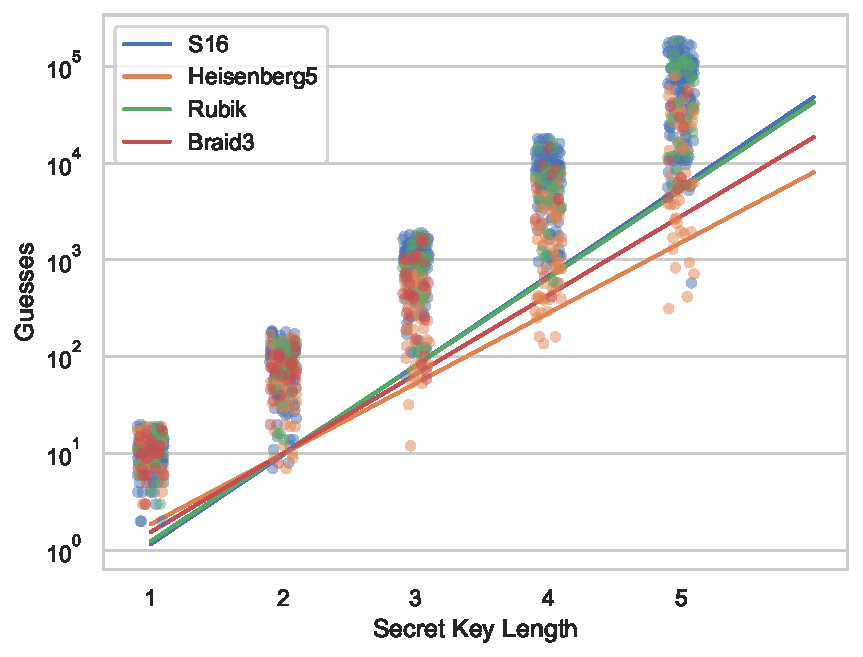
\includegraphics[width=\columnwidth]{images/Guesses-L.pdf}
  \caption{Comparison between groups with respect to number of guesses needed to obtain the shared key using the brute-force algorithm. Each group's performance is measured for various private key lengths, with public set size fixed at 5.}
  \label{fig:guess-l}
\end{figure}

\subsubsection{Relative Lengths}\label{sec:eval-relative-lengths}

Preliminary analysis showed that the average proportion of guesses made by the brute-force algorithm before it found a key \textit{decreases} as we increase the number of private key factors ($L$), for a fixed public key size ($N$). To investigate this, we hold fixed the size of the search space, and vary the values (namely, $L$ and $N$) that determine this size. The naive search space is size $(2N)^L$, so we must choose $N_1 \neq N_2$ and $L_1 \neq L_2$ satisfying the equality $(2N_1)^{L_1} = (2N_2)^{L_2}$. In Figure \ref{fig:fix-keyspace}, we use $(2 \cdot 2)^{2 L_2} = (2 \cdot 8)^{L_2}$, for $L_2 = 2, 3, ..., 7$.

\begin{figure}[hbt]
  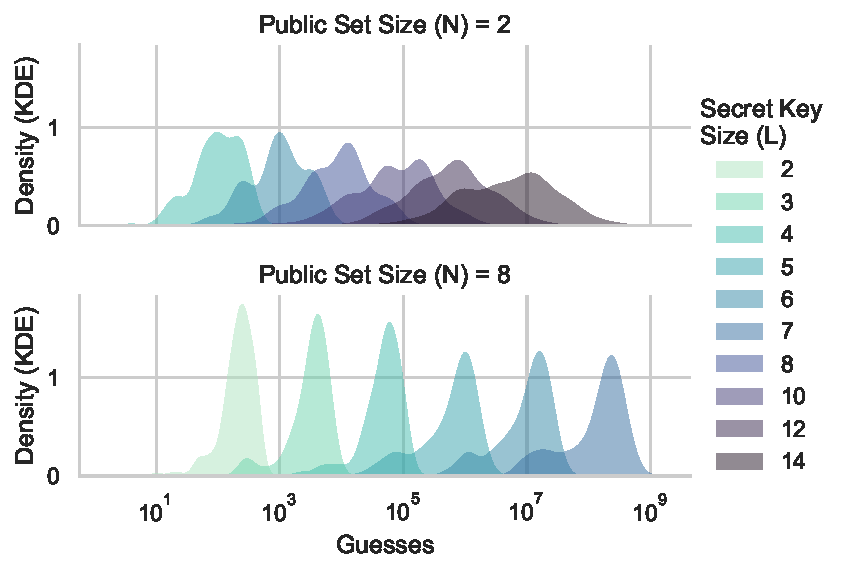
\includegraphics[width=\columnwidth]{images/constant-key-space.pdf}
  \caption{Density of guesses needed to obtain the shared key using the brute-force algorithm, against private keys of $L$ factors. Search space is comparable between the upper and lower graphs, which show different public set sizes $N$ (see Section \ref{sec:eval-relative-lengths}). Platform: $S_{16}$; 100 samples per curve.}
  \label{fig:fix-keyspace}
\end{figure}

The results from this test corroborate the initial observation: on brute-force, the average number of iterations required is much (and more consistently) higher when $N$ is bigger than $L$, even for equally sized search spaces. Curves in the lower graph in Figure \ref{fig:fix-keyspace} showing the larger public set size are all right-leaning. Compare this to the curves in the upper graph showing the smaller public set size (with larger secret keys). The upper graph curves are less agressively right-leaning, meaning that it is easier to brute force longer secret keys chosen from small public sets than it is to brute force short secret keys chosen from larger sets. 

Looking solely at the growth of the naive search space would suggest that Alice and Bob, constrained by a finite cost per exchange, can maximize their security by using very long private keys. After all, private key size is exponentially related to the number of permutations, whereas public set size only reflects the base of the exponent. On the contrary, this result indicates that security is actually favorable when public set size exceeds the number of private key factors. Running an identical test using the Rubik's Cube group as platform yields the same confirmation.

We explain this result by analogy. Consider searching an undirected graph representing the key space of a specific group. It is possible that multiple permutations of group elements multiply to reach the same value, so some nodes in the graph may be more connected than others. The graph exists in $N$ dimensions, as we have ammended the AAG protocol\footnote{See Section \ref{sec:bg-protocol} and related footnote.}, prohibiting public sets from containing any two elements in the same dimension.

In this situation, private key size is analogous to search depth, and public set size relates to the breadth that must be explored. Maximizing one of these factors while holding the other small produces a less than maximal search boundary. If some nodes in the graph are much more connected than others, increasing search depth without increasing breadth only serves to increase the number of times that you visit these highly connected nodes. The presence of these over-represented nodes explains the behavior in Figure \ref{fig:fix-keyspace}. Likewise, having breadth without depth only makes a certain border set of the nodes possible as destinations, limiting key entropy.

The topology of this graph for a given $N$ and $L$ depends on the structure of the chosen platform group, as well as the constituent elements of the public set and private key.